%!TEX program = uplatex
\documentclass[dvipdfmx]{ujarticle}

\usepackage{amsmath}
\usepackage{amssymb}
\usepackage{amsthm}
\usepackage{bm}
\usepackage{eucal}
\usepackage{pdfpages}
\usepackage{tikz}

\theoremstyle{definition}
\newtheorem{dfn}{Definition}[section]
\newtheorem{thm}[dfn]{Theorem}
\newtheorem*{rem}{Remark}
\newtheorem{prop}[dfn]{Proposition}
\newtheorem{cor}[dfn]{Corollary}
\newtheorem*{ex}{Example}
\newtheorem{lem}[dfn]{Lemma}
\def\labelenumi{(\theenumi)}

\setlength{\textwidth}{\paperwidth}
\addtolength{\textwidth}{-40truemm}
\setlength{\textheight}{\paperheight}
\addtolength{\textheight}{-45truemm}
%余白の調節
\setlength{\topmargin}{-10.4truemm}
\setlength{\evensidemargin}{-5.44truemm}
\setlength{\oddsidemargin}{-5.44truemm}
\setlength{\headheight}{17pt}
\setlength{\headsep}{10mm}
\addtolength{\headsep}{-17pt}
\setlength{\footskip}{5mm}

\begin{document}
%\fontsize{9pt}{14pt}\selectfont

\includepdf{../cover/cover.pdf}

\clearpage

\tableofcontents
\clearpage
\section{導入}\label{intro}
幾何群論について語る。\\

Švarc-Milnor Lemma とは,「群が“よい”距離空間によい群作用をしているとき,その群の有限生成系が分かり,群の構造と空間の構造が“大雑把に”等しい」という主張であり,その内容から「幾何学的群論の基本補題」とも言われている.一般に,群が与えられたとき,その群が有限生成であるかどうかの判別は難しいのだが,この補題では生成系が分かるだけでなく,作用している空間の持つ構造と,群の持つ構造が大雑把に等しいことまで分かる.群のことを知りたければ,よく知られている距離空間への作用を考えればよく,逆に距離空間のことを知りたければ,よく知られている群の作用を考えればよい.まさに群と幾何を繋ぐ補題であるといえるだろう.\\

(もうちょい書きたい)

\section{準備}
\subsection{Quasi-Isometry of Meric Spaces}\label{subsec_QI_of_Metric}
この節では,空間同士を見積もるための道具となる写像について述べる.条件の厳しい等長写像から始まり,その条件を少しずつ緩めることによって,幾何学的群論における“大雑把な視点”を得ることができる.

以下,$(X,d_X)$ を距離空間とし,省略して $X$ と表記する.
\begin{dfn}\label{isom}
写像 $f\colon X\rightarrow Y$ が \textbf{等長埋め込み (isometric embedding)} であるとは,任意の $x,x^\prime\in X$ に関して,$d_X(x,x^\prime)=d_Y(f(x),f(x^\prime))$ が成り立つことをいう.また,$f$ が \textbf{等長写像 (isometry)} であるとは,以下の二条件を満たすときをいう.
\begin{enumerate}
  \item $f$ が等長埋め込みである.
  \item ある等長埋め込み $g\colon Y\rightarrow X$ が存在し,$f\circ g=\mathrm{id}_Y,g\circ f=\mathrm{id}_X$ を満たす.
\end{enumerate}
さらに,二つの距離空間 $X,Y$ が \textbf{等長 (isometric)} であるとは,等長写像 $f\colon X\rightarrow Y$ が存在するときをいう. 
\end{dfn}

\begin{rem}
 定義より,等長埋め込みならば単射な連続写像である.よって,等長写像は同相写像である.また,等長埋め込みは全射性を満たすと等長写像となる.
\end{rem}

\begin{dfn}\label{bi-Lip}
写像 $f\colon X\rightarrow Y$ が \textbf{bilipschitz埋め込み (bilipschitz embedding)} であるとは,ある定数 $c\in\mathbb{R}_{>0}$ が存在し,任意の $x,x^\prime\in X$ に対して,
 $$\frac{1}{c}d_X(x,x^\prime)\leq d_Y(f(x),f(x^\prime))\leq cd_X(x,x^\prime)$$
 が成り立つことをいう.また,$f$ が \textbf{bilipschitz equivalence} であるとは,以下の二条件を満たすときをいう.
 \begin{enumerate}
   \item $f$ がbilipschitz埋め込みである.
   \item あるbilipschitz埋め込み $g\colon Y\rightarrow X$ が存在し,$f\circ g=\mathrm{id}_Y$,$g\circ f=\mathrm{id}_X$ を満たす.
 \end{enumerate}
さらに,二つの距離空間 $X,Y$ が \textbf{bilipschitz equivalent} であるとは,bilipschitz equivalence な写像 $f\colon X\rightarrow Y$ が存在するときをいう. 
\end{dfn}

\begin{ex}
通常の距離が入った距離空間 $\mathbb{Z},2\mathbb{Z}$ に対し, $f\colon\mathbb{Z}\rightarrow 2\mathbb{Z}$ を,$f(n)=2n$ とすると,これは等長埋め込みではないが bilipschitz埋め込みである.実際,この写像は $c=2$ とすれば bilipschitz埋め込み の定義を満たす.また,$g\colon2\mathbb{Z}\rightarrow \mathbb{Z}$ を,$g(m)=m/2$ とすれば,$f,g$ によって $\mathbb{Z}$ と $2\mathbb{Z}$ は bilipschitz equivalent である.
\end{ex}

\begin{rem}
bilipschitz埋め込み は単射な連続写像である.よって,bilipschitz equivalence は同相写像である.また,bilipschitz埋め込み は全射性を満たすと bilipschitz equivalence となる.
\end{rem}

\begin{dfn}
写像 $f\colon X\rightarrow Y$ が 写像 $f^\prime\colon X\rightarrow Y$ から\textbf{finite distance} であるとは,ある定数$c\in\mathbb{R}_{>0}$ が存在し,任意の $x\in X$ に対して,
 $$d_Y(f(x),f^\prime(x))\leq c$$
が成り立つことをいう.
\end{dfn}

\begin{dfn}\label{QI}
写像 $f\colon X\rightarrow Y$ が \textbf{擬等長埋め込み (quasi-isometric embedding)} であるとは,ある定数 $c\in\mathbb{R}_{>0}$,$b\in\mathbb{R}_{\geq0}$ が存在し,任意の $x,x^\prime\in X$ に対して,
 $$\frac{1}{c}d_X(x,x^\prime)-b\leq d_Y(f(x),f(x^\prime))\leq cd_X(x,x^\prime)+b$$
 が成り立つことをいう.このとき,$f$ を \bm{$(c,b)$}\textbf{-quasi-isometric embedding} とも表現する.また,$f$ が\textbf{擬等長写像 (quasi-isometry, QI)} であるとは,以下の二条件を満たすときをいう.
 \begin{enumerate}
  \item $f$ が擬等長埋め込みである.
  \item ある擬等長埋め込み $g\colon Y\rightarrow X$ が存在し,
  $f\circ g$ が $\mathrm{id}_Y$ と finite distance,$g\circ f$ が $\mathrm{id}_X$ と finite distance である.
 \end{enumerate}
さらに,二つの距離空間 $X,Y$ が \textbf{擬等長 (quasi-isometric)} であるとは,擬等長写像 $f\colon X\rightarrow Y$ が存在するときをいう.
\end{dfn}

\begin{ex}
通常の距離が入った距離空間 $\mathbb{R},\mathbb{Z}$ に対し, $f\colon\mathbb{R}\rightarrow\mathbb{Z}$ を,$f(x)=\lfloor x \rfloor$ と定めると,これは bilipschitz embedding ではないが,擬等長埋め込みである.実際,この写像は $c=1,b=1$ とすれば擬等長埋め込みの定義を満たす.また,$\mathbb{Z}$ から $\mathbb{R}$ への包含写像を考えると,$f$ と包含写像によって $\mathbb{Z}$ と $\mathbb{R}$ は擬等長である.
\end{ex}

\begin{rem}
擬等長埋め込みは連続とは限らない(実際上の例の $f$ は連続でない).同様に,擬等長写像は連続であるとは限らない.
\end{rem}

\begin{figure}[h]
\centering
\includegraphics[width=8cm]{../picture/benzu}
\caption{各写像の関係}
\end{figure}

\begin{rem}
  等長埋め込み同士の合成写像は等長埋め込みであり,bilipschitz埋め込み同士の合成写像はbilipschitz埋め込みであり,擬等長埋め込み同士の合成は擬等長埋め込みである.
\end{rem}

定数倍と定数分のズレを許してしまうという,擬等長の“大雑把な視点”が幾何学的群論では大切なのだが,その擬等長に関する定義について,それと同値なものを紹介する.

\begin{prop}\label{dense image}
Definition \ref{QI} の 擬等長写像における二条件は,以下の二条件と同値.
\begin{enumerate}
  \item[[1]] $f$ が擬等長埋め込みである.
  \item[[2]] ある定数 $c\in\mathbb{R}_{>0}$ が存在し,任意の $y\in Y$ に対してある $x\in X$ をとると,$d_Y(f(x),y)\leq c$ を満たす.
\end{enumerate}
\end{prop}

\begin{proof}
Definition \ref{QI} を満たすならば[1],[2]を満たすことの証明:\\
[2]を示せばよい.$f\colon X\rightarrow Y$ に対し,定義より,ある擬等長写像 $g\colon Y\rightarrow X$ が存在し,$f\circ g$ が $\mathrm{id}_Y$ と finite distance である.任意の $y\in Y$ をとる.$x:=g(y)$ と定めることで,
$$d_Y(f(x),y)=d_Y((f\circ g)(y),y)\leq c$$
を満たす.\\
[1],[2]を満たすならば Definition \ref{QI} を満たすことの証明:\\ 
仮定より,ある定数 $c\in\mathbb{R}_{>0}$ が存在し,
\begin{enumerate}
  \item 任意の $x,x^\prime \in X$ に対し,$\frac{1}{c}d_X(x,x^\prime)-c \leq d_Y(f(x),f(x^\prime)) \leq cd_X(x,x^\prime)+c.$\label{1}
  \item 任意の $y\in Y$ に対しある $x\in X$ が存在し,$d_Y(f(x),y)\leq c.$\label{2}
\end{enumerate}
\eqref{2} と選択公理を用いて,$y\in Y$ に対し,$d_Y(f(x_y),y)\leq c$ を満たすような $x_y\in X$ を選ぶ. 写像 $g\colon Y\rightarrow X$ を,$y\mapsto x_y$ と定めると,$g\circ f$,$f\circ g$ ともに finite distance となる.実際に,任意の $x\in X$ に対して,
\begin{align*}
  d_X((g\circ f)(x),x)&=d_X(x_{f(x)},x)\\
  &\leq c\cdot d_Y(f(x_{f(x)}),f(x)) +c^2\\
  &\leq c\cdot c +c^2=2c^2
\end{align*}
となる.$f\circ g$ に関しても,任意の $y\in Y$に対して,
\begin{align*}
  d_Y((f\circ g)(y),y)=d_Y(f(x_y),y)\leq c
\end{align*}
が成立する.
\end{proof}

\begin{dfn}
Proposition \ref{dense image} の条件[2]を $f$ が満たすとき,$f$ は \textbf{quasi-dense image} をもつという.
\end{dfn}

\subsection{Quasi-Isometry of Groups}
\ref{subsec_QI_of_Metric} 節では距離空間同士を大雑把にみることについて述べたが,本節では群を距離空間に拡張し,群に対しても定義を行う.

以下,$G$ を群として,$S$ をその生成系とする.
\begin{dfn}
生成系 $S$ による,群 $G$ 上の \textbf{word metric} とは,$d_S\colon G\times G\rightarrow \mathbb{N}$,
 $$d_S(g,h):=\mathrm{min}\{n\in\mathbb{N}\mid s_1,s_2,\ldots, s_n\in S\cup S^{-1},g^{-1}h=s_1s_2\cdots s_n\}$$
であり,これは $G$ 上の距離関数である.
\end{dfn}

\begin{ex}
  群 $G$ の生成系 $S$ からなる $\mathrm{Cay}(G,S)$ において,グラフ上の頂点間の距離とはまさに $d_S$ のことである($\mathrm{Cay}(G,S)$ の定義は Definition \ref{cayley} を参照されたい).
\end{ex}

\begin{dfn}\label{GQIX}
$G$ を有限生成群としたとき,$G$ が距離空間 $X$ に \textbf{bilipschitz equivalent} であるとは,$G$ のある有限な生成系 $S$ がとれ,距離空間 $(G,d_S)$ と $X$ が bilipschitz equivalent であることをいう.また,$G$ が $X$ に \textbf{擬等長 (quasi-isometric)} であるとは,ある有限な生成系 $S$ がとれ,距離空間 $(G,d_S)$ と $X$ が,quasi-isometric であることをいう.
\end{dfn}

\begin{rem}
  群 $G$ とその生成系 $S$ からできる距離空間 $(G,d_S)$ では,$G$ が有限生成であること,$S$ を有限としていることに注意.
\end{rem}

\begin{ex}
  群 $\mathbb{Z}^2$ とその生成系 $S=\{(0,1),(1,0)\}$ からなる距離空間 $(\mathbb{Z}^2,d_S)$ は,距離空間 $\mathbb{R}^2$ と擬等長である.
\end{ex}

群に組み込む距離関数を word metric にした場合,その定義からこれは生成系に大きく依存するため,距離空間と群が同じ構造を持つかどうかの議論が難しくなる.しかし,擬等長という“大雑把な視点”で見ると,生成系に依らずに議論することが可能である.

\begin{prop}\label{Sprime}
  $S$,$S^\prime$ をともに群 $G$ の有限な生成系 としたとき,距離空間 $(G,d_S)$ が 距離空間 $(X,d_X)$ と $f$ で bilipschitz equivalent ならば,$(G,d_{S^\prime})$ と $(X,d_X)$ も $f$ で bilipschitz equivalent である.
\end{prop}

\begin{proof}
$f \colon (X,d_X)\rightarrow (G,d_S)$,$f^\prime\colon (X,d_X)\rightarrow (G,d_{S^\prime})$ を共に bilipschitz equivalence とすると,可換図式
\begin{center}
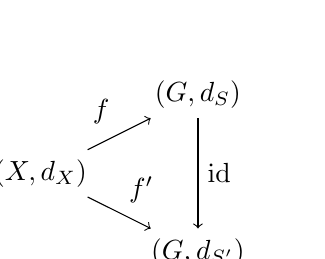
\begin{tikzpicture}[auto]
\node (X) at (0, 0) {$(X,d_X)$};
\node (S) at (2, 1) {$(G,d_S)$};
\node (S*) at (2, -1) {$(G,d_{S^\prime})$};
\draw[->] (X) to node {$f$} (S);
\draw[->] (X) to node {$f^\prime$} (S*);
\draw[->] (S) to node {id} (S*);
\end{tikzpicture}
\end{center}
より,$f^\prime=f\circ\mathrm{id}=f$ が成立する.bilipschitz equivalence の合成写像は bilipschitz equivalence なので,あとは $\mathrm{id}$ が bilipschitz equivalence であることを示せばよい.$c$ を,
$$c:=\underset{s\in S\cup S^{-1}}{\mathrm{max}}d_{S^\prime}(e,s)$$
とすると,$S$ は有限なのでこれは有限値である.$g,h\in G$ をとり,$d_S(g,h)=n$ とし,$g^{-1}h=s_1s_2\cdots s_{n-1} s_n$ ($s_1,s_2,\ldots,s_{n-1},s_n\in S\cup S^{-1}$) と表せられるとする.このとき,$S^\prime$ 上での $g,h$ の word metric は,
\begin{align*}
  d_{S^\prime}(g,h)&=d_{S^\prime}(g,s_1s_2\cdots s_nh)\\
  &\leq d_{S^\prime}(g,gs_1)+d_{S^\prime}(gs_1,gs_1s_2)+\cdots+d_{S^\prime}(gs_1s_2\cdots s_{n-1},gs_1s_2\cdots s_{n-1}s_n)\\
  &=d_{S^\prime}(e,s_1)+d_{S^\prime}(e,s_2)+\cdots+d_{S^\prime}(e,s_{n-1})+d_{S^\prime}(e,s_n)\\
  &\leq c+c+\cdots+c+c\\
  &=cn=cd_S(g,h)
\end{align*}
となり,$d_{S^\prime}(g,h)\leq cd_S(g,h)$ が得られる.同様の議論を $S,S^\prime$ を逆にしてすれば $d_S(g,h)\leq cd_{S^\prime}(g,h)$ が得られる.id は全単射であることも含めると,id は bilipschitz equivalence である.
\end{proof}

\begin{rem}
  Definition \ref{GQIX} と Proposition \ref{Sprime} より,距離空間に bilipschitz equivalent な群(quasi-isometric な群)は,その(有限)生成系の取り方に依らない.
\end{rem}

\subsection{Quasi-Geodesic}
本節では,\ref{intro} 章でも記した,“よい”距離空間について述べる.
\begin{dfn}
距離空間 $X$ 上の長さ $L\in\mathbb{R}_{>0}$ の \textbf{測地線 (geodesic)} とは,$[0,L]\subset\mathbb{R}$ から $X$ への等長埋め込み,$\gamma\colon[0,L]\rightarrow X$ のことである.また,$X$ が \textbf{測地的 (geodesic)} であるとは,任意の $x,x^\prime\in X$ において,$\gamma(0)=x$,$\gamma(L)=x^\prime$ となるような 等長埋め込み $\gamma$ がとれるときをいう.
\end{dfn}

\begin{ex}
$\mathbb{R}^n$ は測地的だが,$\mathbb{R}^n\setminus\{0\}$ は測地的でない.実際,$(1,0)$ と $(-1,0)$ 間の距離は $2$ だが,この測地線は原点を通ってしまう.一般に,$\mathbb{R}^n$ 上の凸集合は測地的である.
\end{ex}

\begin{dfn}
距離空間 $X$ 上の \textbf{\bm{$(c,b)$}-擬測地線 (\bm{$(c,b)$}-quasi-godesic)} とは,とは,$[0,L]\subset\mathbb{R}$ から $X$ への $(c,b)$-擬等長埋め込み,$\gamma\colon[0,L]\rightarrow X$ のことである.また,$X$ が \textbf{\bm{$(c,b)$}-擬測地的 (\bm{$(c,b)$}-quasi-godesic)} であるとは,任意の $x,x^\prime\in X$ において,$\gamma(0)=x$,$\gamma(L)=x^\prime$ となるような $(c,b)$-擬等長埋め込み,$\gamma$ がとれるときをいう.また,$(c,b)$ を省略し,単に擬測地線や擬測地的ともいう.
\end{dfn}

\begin{ex}
$\mathbb{R}^n\setminus\{0\}$ は,$(1,\epsilon)$-測地的である($\epsilon>0$).これは,原点中心で十分小さい半径の円で原点を迂回すれば,擬測地線が得られるからである.
\end{ex}

\section{主定理}
本論文の主定理となる,Švarc-Milnor Lemma と,それに関連する主張について紹介する.
\subsection{Švarc-Milnor Lemma}
\begin{thm}\label{svarc}
$G$ を群とし,$(c,b)$-測地的な距離空間 $(X,d)$ 上に等長な群作用があるとする.もしある部分集合 $B\subset X$ が存在し,
   \begin{enumerate}
   \item[(a)] $\mathrm{diam}B:=\underset{x,y\in B}{\mathrm{sup}}d(x,y)<\infty,$
   \item[(b)] $\bigcup_{g\in G}g\cdot B=X,$
   \item[(c)] 集合 $S:=\{g\in G\mid g\cdot B^\prime \cap B^\prime \neq \emptyset\}$ が有限.
   \end{enumerate}
 を満たすならば,
 \begin{enumerate}
  \item $S$ は $G$ の有限生成系である.\label{S_is_generating_set}
\item 任意の $x\in X$ に対して定まる写像 $\varphi\colon G\rightarrow X\;;\; g\mapsto gx$ によって,$G$ と $X$ は擬等長.\label{G~X}
 \end{enumerate}
ただし,$B^\prime :=\{x\in X\mid y\in X,d_X(x,y)\leq 2b\}$ と定める.
\end{thm}

\begin{proof}
\eqref{S_is_generating_set} の証明:\\
$g\in G$ を任意にとる.$x\in B$ としたとき,$X$ の仮定から $\gamma(0)=x$,$\gamma(L)=g\cdot x$ なる $(c,b)$-擬測地線 $\gamma$ が存在する.$[0,L]$ をおおよそ $n:=\lceil L\cdot c/b \rceil$ 等分した点列を $t_i (0\leq i\leq n)$ とする.厳密には,
$$t_i:=i\cdot b/c\;(0\leq i\leq n-1),t_n:=L$$
と定める.この点列と対応するように,$\mathrm{Im}\gamma$ に点列 $x_i \in X (0\leq i \leq n)$ をとる.つまり,
$$x_i:=\gamma(t_i) (0\leq i\leq n)$$
である.$B$ の仮定より,各 $x_i$ に対して,$x_i\in g_i\cdot B$ となるような $g_i\in G$ を選ぶことができる(図\ref{syoumei}参照).

\begin{figure}[h]
\centering
\includegraphics[width=17cm]{../picture/syoumei}
\caption{$t_i,x_i,g_i$ の関係}
\label{syoumei}
\end{figure}

\noindent
ここで,$g_0=e$,$g_n=g$ としておく.$\gamma$ は $(c,b)$-擬測地線 なので,不等式
$$d(x_{i-1},x_i)\leq c|t_{i-1}-t_i|+b=c\cdot b/c+b=2b$$
を得る.等長に群作用をしていることに注意すると,
\begin{align*}
  x_i & \in\{x\in X\mid y\in g_{i-1}\cdot B,d_X(x,y)\leq 2b\}\\
  &=\{x\in X\mid g^{-1}_{i-1}\cdot y\in B,d_X(g^{-1}_{i-1}\cdot x,g^{-1}_{i-1}\cdot y)\leq 2b\}\\
  &=g_{i-1}\cdot\{x^\prime\in X\mid y^\prime\in B,d_X(x^\prime,y^\prime)\leq 2b\}\\
  &=g_{i-1}\cdot B^\prime
\end{align*}
を得る.$x_i\in g_i\cdot B \subset g_i\cdot B^\prime$ でもあるので,
\begin{align*}
  g_i\cdot B^\prime \cap g_{i-1}\cdot B^\prime &\neq\emptyset,\\
  (g_{i-1}^{-1}\cdot g_i)\cdot B^\prime \cap B^\prime &\neq \emptyset.
\end{align*}
よって,$(g_{i-1})^{-1}\cdot g_i \in S$ であり,$s_i:=(g_{i-1})^{-1}\cdot g_i\in S$ とすれば, $g$ は $g=g_n=e(g_0^{-1}g_1)(g_1^{-1}g_2)\cdots(g_{n-1}^{-1}g_n)=es_1s_2\cdots s_n$ と $S$ の元で表すことができる.\\

\eqref{2} の証明:\\
$B$ の仮定より,任意の $x\in X$ は $B$ に含まれていると考えてよい($x\in g\cdot B$ となる $g\cdot B$ を改めて $B$ とすればよいため).
\begin{enumerate}
  \item[[1]] 写像 $\varphi(g)=g\cdot x$ に関して,quasi-dense image であること.
  \item[[2]] 擬等長埋め込みであること.
\end{enumerate}
の二点を示す.\\

\noindent
[1] $\varphi$ が quasi-dense image であること:\\
任意の $x^\prime \in X$ に関して,$x^\prime\in g^\prime\cdot B$ となる $g^\prime \in G$ がとれるため,
$$d_X(x^\prime,\varphi(g^\prime))=d_X(x^\prime,g^\prime\cdot x)\leq \mathrm{diam}(g^\prime \cdot B)=\mathrm{diam}B.$$
仮定より $\mathrm{diam}B$ は有限なので,$\varphi$ が quasi-dense image であることが示された.\\

\noindent
[2] $\varphi$ が 擬等長埋め込みであること:\\
ある定数 $C>0,B\geq0$ が存在し, 任意の $g,h\in G$ に対して,
$$\frac{1}{C}d_S(g,h)-B\leq d_X(\varphi(g),\varphi(h))\leq Cd_S(g,h)+B.$$
であることを示せばいいが,word metric の定義と $G$ が等長に作用していることから,
\begin{align*}
  d_S(g,h)&=d_S(e,g^{-1}h)\\
  d_X(\varphi(g),\varphi(h))&=d_X(g\cdot x,h\cdot x)\\
  &=d_X(x,(g^{-1}h)\cdot x)\\
  &=d_X(\varphi(e),\varphi(g^{-1}h))
\end{align*}
が成立する.以上より,ある定数 $C>0,B\geq 0$ が存在し, 任意の $g\in G$ に対して,
$$\frac{1}{C}d_S(e,g)-B\leq d_X(\varphi(e),\varphi(g))\leq Cd_S(e,g)+B$$
が成立することを示せばよい.\\

\noindent
[$2-1$] $\frac{1}{C}d_S(e,g)-B\leq d_X(\varphi(e),\varphi(g))$ が成立すること:\\
 任意に $g\in G$ をとる.このとき,$g$ に対して proof of (1) と同様の議論により $s_1,s_2,\ldots ,s_n\in S\cup S^{-1}$ がとれ,$g=s_1s_2\cdots s_n$ と表せられる.このときの $\gamma$ を用いて,
\begin{align*}
  d_X(\varphi(e),\varphi(g))=d_X(x,g\cdot x)&=d_X(\gamma(0),\gamma(L))\\
  &\geq \frac{1}{c}L-b\\
  &\geq \frac{1}{c}\frac{b(n-1)}{c}-b=\frac{b}{c^2}n-b-\frac{b}{c^2}\\
  &\geq \frac{1}{c^2}d_S(e,g)-b-\frac{b}{c^2}
\end{align*}
とすることで,下からの不等式が得られる.\\

\noindent
[$2-2$] $d_X(\varphi(e),\varphi(g))\leq Cd_S(e,g)+B$ が成立すること:\\
任意に $g\in G$ をとる.$d_S(e,g)=n$ とし,$g=s_1s_2\cdots s_n$ と表せられるとする.このとき,各 $s_i\in S\cup S^{-1}$ ($1\leq i\leq n$) に対して,$S$ の定義 $B^\prime\cap s_i\cdot B^\prime\neq\emptyset$ より,
$$d_X(x,s_i\cdot x)\leq \mathrm{diam}B+2b+\mathrm{diam}B=2(\mathrm{diam}B+b)$$
が成立する(図 \ref{2diamB+2b} 参照).

\begin{figure}[h]
\centering
\includegraphics[width=12cm]{../picture/2diamB+2b}
\caption{$d_X(x,s_i\cdot x)$ の不等式}
\label{2diamB+2b}
\end{figure}

\noindent
これより,
\begin{align*}
  d_X(\varphi(e),\varphi(g))=d_X(x,g\cdot x)&=d_X(x,s_1s_2\cdots s_nx)\\
  & \leq d_X(x,s_1x)+d_X(s_1x,s_1s_2x)+\cdots+d_X(s_1s_2\cdots s_{n-1}x,s_1s_2\cdots s_nx)\\
  & = d_X(x,s_1x)+d_X(x,s_2x)+\cdots+d_X(x,s_nx)\\
  & \leq 2(\mathrm{diam}B+b)\cdot n\\
  & =2(\mathrm{diam}B+b)\cdot d_S(e,g)
\end{align*}
を得る.
\end{proof}

\begin{ex}
通常の距離が入った距離空間 $\mathbb{R}^2$ に群 $\mathbb{Z}^2$ が,
\begin{align*}
  (1,0)\cdot (x,y) = (x+2,y)\\
  (0,1)\cdot (x,y) = (x,y+2)
\end{align*}
からなる作用をしているとする.作用の仕方からこれは等長な群作用である.$\mathbb{R}^2$ を $(1,1/2)$-擬測地的空間とし,部分集合 $B\subset \mathbb{R}^2$ を,
$$B=\{(x,y)\in\mathbb{R}^2\mid -1\leq x\leq 1,-1\leq y\leq 1\}$$
とすれば,これは Theorem\ref{svarc} の条件(a),(b)を満たす.$S\subset \mathbb{Z}^2$ は,
\begin{align*}
  S&=\{g\in\mathbb{Z}^2\mid g\cdot B^\prime\cap B^\prime\neq \emptyset\}\\
  &=\{-2,-1,0,1,2\}\times\{-2,-1,0,1,2\}
\end{align*}
となり,条件(c)を満たす.よって,Theorem \ref{svarc} より,$\mathbb{Z}^2$ は $S$ によって生成され,$\mathbb{R}^2$ と $\mathbb{Z}^2$ は擬等長である.

\begin{figure}[h]
\centering
\includegraphics[width=10cm]{../picture/R2Z2}
\caption{$B,B^\prime$ の図}
\label{R2Z2}
\end{figure}

\end{ex}
\subsection{Švarc-Milnor Lemma の拡張}
Theorem \ref{svarc} は,群作用が等長でなくても成立する.つまり,以下のとおりである.
\begin{thm}
  Theorem \ref{svarc} は,群 $G$ が距離空間 $X$ に等長な群作用だけでなく,擬等長な群作用としても成り立つ.
\end{thm}
証明は,以下のLemma \ref{lem1}--\ref{lem3} より与えらえる.

\begin{lem}\label{lem1}
  Theorem \ref{svarc} の証明において,群作用が $(c^\prime,b^\prime)$-擬等長な作用でも $x_i\in g_{i-1}\cdot B^\prime$ が成立する.ただし,$B^\prime :=\{x\in X\mid y\in X,d_X(x,y)\leq 2bc^\prime+b^\prime\}$ とする.
\end{lem}
\begin{proof}
  群作用が $(c^\prime,b^\prime)$-擬等長なので,
  $$\frac{1}{c^\prime}d_X(g\cdot x,g\cdot y)-\frac{b^\prime}{c^\prime}\leq d_X(x,y)$$
  が成立する.したがって,
  \begin{align*}
    x_i & \in\{x\in X\mid y\in g_{i-1}\cdot B,d_X(x,y)\leq 2b\}\\
    &\subset \{x\in X\mid g^{-1}_{i-1}\cdot y\in B,\frac{1}{c^\prime}d_X(g^{-1}_{i-1}\cdot x,g^{-1}_{i-1}\cdot y)-\frac{b^\prime}{c^\prime}\leq 2b\}\\
    &=\{x\in X\mid g^{-1}_{i-1}\cdot y\in B,d_X(g^{-1}_{i-1}\cdot x,g^{-1}_{i-1}\cdot y)\leq 2bc^\prime+b^\prime\}\\
    &=g_{i-1}\cdot\{x^\prime\in X\mid y^\prime\in B,d_X(x^\prime,y^\prime)\leq 2bc^\prime+b^\prime\}\\
    &=g_{i-1}\cdot B^\prime
  \end{align*}
  を得る.
\end{proof}

\begin{lem}\label{lem2}
  Theorem \ref{svarc} の証明において,群作用が $(c^\prime,b^\prime)$-擬等長な作用でも $\mathrm{diam}(g^\prime\cdot B)< \infty$ である. 
\end{lem}
\begin{proof}
   群作用が $(c^\prime,b^\prime)$-擬等長なので,
      $$d_X(g\cdot x,g\cdot y)\leq c^\prime d_X(x,y)+b^\prime$$
    が成立する.よって,
  \begin{align*}
    \mathrm{diam}(g^\prime\cdot B)&=\underset{x,y\in g^\prime\cdot B}{\mathrm{sup}}d_X(x,y)\\
    &=\underset{x^\prime,y^\prime\in B}{\mathrm{sup}}d_X(g\cdot x^\prime,g\cdot y^\prime)\\
    &\leq \underset{x^\prime,y^\prime\in B}{\mathrm{sup}} c^\prime d_X(x^\prime,y^\prime)+b^\prime\\
    &\leq c^\prime \mathrm{diam}B+b^\prime
  \end{align*}
    となり,$\mathrm{diam}(g^\prime\cdot B)$ は有限値.
\end{proof}

\begin{lem}\label{lem3}
  Theorem \ref{svarc} の証明において,群作用が $(c^\prime,b^\prime)$-擬等長な作用でも,定数$C>0,B\geq 0$ があり,任意の $g,h\in G$ に関しての不等式
  $$\frac{1}{C}d_S(e,g)-B\leq d_X(\varphi(e),\varphi(g))\leq Cd_S(e,g)+B$$
  が成立するならば,定数$C^\prime>0,B^\prime\geq 0$ があり,任意の $g,h\in G$ に関しての不等式
  $$\frac{1}{C^\prime}d_S(g,h)-B^\prime\leq d_X(\varphi(g),\varphi(h))\leq C^\prime d_S(g,h)+B^\prime$$
  が成立する.
\end{lem}
\begin{proof}
word metric の定義から,
\begin{align}
  d_S(g,h)&=d_S(e,g^{-1}h)\label{lem3.5.1}
\end{align}
が成立し,群作用が$(c^\prime,b^\prime)$-擬等長なことから,
\begin{align}
  d_X(\varphi(e),\varphi(g^{-1}h))&=d_X(x,(g^{-1}h)\cdot x)\nonumber\\
  &\leq c^\prime d_X(g\cdot x,h\cdot x)+c^\prime b^\prime=c^\prime d_X(\varphi(g),\varphi(h))+c^\prime b^\prime\label{lem3.5.2}\\
  d_X(\varphi(e),\varphi(g^{-1}h))&=d_X(x,(g^{-1}h)\cdot x)\nonumber\\
  &\geq\frac{1}{c^\prime}d_X(g\cdot x,h\cdot x)-\frac{b^\prime}{c^\prime}=\frac{1}{c^\prime}d_X(\varphi(g),\varphi(h))-\frac{b^\prime}{c^\prime}\label{lem3.5.3}
\end{align}
が成立する.仮定より,以下の不等式
\begin{equation}
\frac{1}{C}d_S(e,g)-B\leq d_X(\varphi(e),\varphi(g))\leq Cd_S(e,g)+B\label{lem3.5.4}
\end{equation}
が成立するので,これらの不等式を用いて,
\begin{align*}
  \frac{1}{C}d_S(g,h)-B&=\frac{1}{C}d_S(e,g^{-1}h)-B \qquad \eqref{lem3.5.1} より\\
  &\leq d_X(\varphi(e),\varphi(g^{-1}h)) \qquad \eqref{lem3.5.4} より\\
  &\leq c^\prime d_X(\varphi(g),\varphi(h))+c^\prime b^\prime \qquad \eqref{lem3.5.2} より\\
  \frac{1}{Cc^\prime}d_S(g,h)-\frac{B+c^\prime b^\prime}{c^\prime}&\leq d_X(\varphi(g),\varphi(h))
\end{align*}
が得られ,もう一方も
\begin{align*}
  Cd_S(g,h)+B&=Cd_S(e,g^{-1}h)+B \qquad \eqref{lem3.5.1} より\\
  &\geq d_X(\varphi(e),\varphi(g^{-1}h)) \qquad \eqref{lem3.5.4} より\\
  &\geq \frac{1}{c^\prime} d_X(\varphi(g),\varphi(h))-\frac{b^\prime}{c^\prime} \qquad \eqref{lem3.5.3} より\\
  Cc^\prime d_S(g,h)+(Bc^\prime +b^\prime)&\geq d_X(\varphi(g),\varphi(h))
\end{align*}
が得られ,目的の不等式が成立する.
\end{proof}


\section{主定理 位相空間論 版}
Theorem \ref{svarc} の主張を,位相空間論の視点で言い換えた主張が存在する.その主張に必要な用語の定義を \ref{subsec_jyunbi} 節で行った後,\ref{subsec_svarc_top} 節にて述べる.
\subsection{準備}\label{subsec_jyunbi}
\begin{dfn}
  距離空間 $(X,d)$ が \textbf{proper} であるとは,任意の $x\in X$,$r\in \mathbb{R}_{>0}$ に関して,集合
  $$\{y\in X\mid d(x,y)\leq r\}$$
  が常にコンパクトになることをいう.
\end{dfn}

\begin{ex}
  ユークリッド空間は proper である一方,$\mathbb{R}$ の部分空間として $(0,1)$ に相対位相を入れた空間は,$(0,1)$ 自身は有界閉集合だがコンパクトでない.また,一つの頂点から無限本の辺が伸びているようなグラフは proper でない.
\end{ex}

\begin{dfn}
 群 $G$ が位相空間 $X$ に作用しているとする.この作用が \textbf{properly discontinuous} であるとは,任意のコンパクトな集合 $K\subset X$ に関して,
 $$\{g\in G\mid g\cdot K\cap K\neq \emptyset\}$$
 が有限集合であることをさす.
\end{dfn}

\begin{ex}
$\mathbb{R}$ に $\mathbb{Z}$ が加法で群作用をしているとき,この作用は properly discontinuous である.しかし,$\mathbb{Q}$ が加法で群作用をしている場合,この作用は properly discontinuous ではない.
\end{ex}

\begin{dfn}
  群 $G$ が位相空間 $X$ に作用しているとする.この作用が \textbf{余コンパクト (cocompact)} であるとは,商空間 $G\backslash X$ がコンパクトであることをいう.言い換えると,あるコンパクトな集合 $K\subset X$ が存在し,
  $$X=\bigcup_{g\in G}g\cdot K$$
  を満たす.
\end{dfn}

\begin{ex}
  $\mathbb{R}$ に $\mathbb{Z}$ や $\mathbb{Q}$ が加法で群作用をしているとき,この作用は余コンパクトである.一方,$\mathbb{R}^2$ に $\mathbb{Z}$ が作用する場合,これは余コンパクトでない(商空間は$S^1\times \mathbb{R}$ と同相であり,これはコンパクトでないため).
\end{ex}

\subsection{Švarc-Milnor Lemma (位相空間論 版)}\label{subsec_svarc_top}
\begin{thm}
  群 $G$ が,proper かつ擬測地的な距離空間 $(X,d)$ に,等長に作用しているとする.この群作用が properly discontinuous かつ余コンパクトであれば,$G$ は有限生成であり,$G$ と $X$ は擬等長である.
\end{thm}
\begin{proof}
$X$ は擬測地的であるので,Thm \ref{svarc} の仮定を満足するような $B\subset X$ をみつければよい.以下,$X$ は $(1,b)$-quasi-geodesic であるとする($b>0$).自然な射影 $\pi\colon X\rightarrow G\backslash X$ は開写像であるので,開球 $B_1(x)=\{y\in X\mid d(x,y)<1\}$ の像 $\pi(B_1(x))$ は $G\backslash X$ 上の開集合である.また,$\pi(X)=G\backslash X$ より,$\{\pi(B_1(x))\}_{x\in X}$ は $G\backslash X$ の開被覆である.$G\backslash X$ のコンパクト性より,これらから有限個 $\{\pi(B_1(x_k))\}_{1\leq k\leq n}$ の開被覆で $G\backslash X$ を覆うことができる.各開球 $B_1(x_k)$ の閉包 $\overline{B_1(x_k)}$ を考え,$$B=\bigcup_{k=1}^n\overline{B_1(x_k)}$$ とすれば,
\begin{enumerate}
  \item[(a)] $\mathrm{diam}B<\infty$.
  \item[(b)] $\bigcup_{g\in G}g\cdot B=X$.
\end{enumerate}
\noindent
をみたす.また,$B$ はコンパクト集合である($X$ の proper 性から各 $\overline{B_1(x_k)}$ はコンパクトであり,$B$ はそれらの有限和のため).同様の議論として,$B^\prime=\{x\in X\mid y\in B,d(x,y)\leq 2b\}$ とすれば,これはコンパクト集合である.そして群作用が properly discontinuous であることから,
 $$\{g\in G\mid g\cdot B^\prime\cap B^\prime\neq \emptyset\}$$
は有限である(c).
\end{proof}

\subsection{応用例}
この定理の応用例として,以下のような主張がある.
\begin{cor}
  コンパクトで境界のないリーマン多様体 $M$ と,その普遍被覆 $\widetilde{M}$ に関して,基本群 $\pi_1(M)$ は有限生成であり,$\tilde{x}\in\widetilde{M}$ によって定まる写像
  $$\pi_1(M)\rightarrow \widetilde{M}\; ;\; g\mapsto g\cdot \tilde{x}$$
  は擬等長写像である.なお、ここでの群作用は被覆変換による群作用とする.
\end{cor}

\begin{proof}
\noindent
($\widetilde{M}$ が proper かつ geodesic な metric space であること)

\noindent
(群作用が isometric であること)

\noindent
(群作用が cocompact であること)
%被覆空間の定義より,$\pi_1(M)\backslash \widetilde{M}$ は $M$ と同相である.仮定より $M$ はコンパクトなので,$\pi_1(M)\backslash \widetilde{M}$ もそうである.\\

\noindent
(群作用が properly discontinuous であること) 
%任意のコンパクトな集合 $K\subset \widetilde{M}$ をとる.有限個の開被覆 $\{\widetilde{U}_k\}_{1\leq k\leq n}$ に関して,被覆変換の一意性により $g\cdot\widetilde{U}_k\cap\widetilde{U}_l$ を満たすような $g\in G$ は,$(k,l)$ のペアに対し高々一個である.したがって,$$g\cdot K\cap K\subset g\cdot(\bigcup_{k=1}^n\widetilde{U}_k)\cap (\bigcup_{k=1}^n\widetilde{U}_k)$$が空でないような $g\in G$ は有限個である.
\end{proof}

\appendix
\section{付録}
ここでは幾何学的群論の分野にて基本的な概念となる Cayleyグラフ や,その周辺の事項について述べる.
\subsection{Cayley Graphs}
以下,$G$ を群として,$S$ をその生成系とする.

\begin{dfn}\label{cayley}
  生成系 $S$ による群 $G$ の \textbf{Cayley graph} とは,以下のようなグラフである.このグラフを $\mathrm{Cay}(G,S)$ と表記する.
  \begin{enumerate}
    \item 頂点集合を $G$ とする.
    \item 辺集合を $\{\{g,g\cdot s\}\mid g\in G,s\in(S\cup S^{-1})\setminus\{e\}\}$ とする.
  \end{enumerate}
\end{dfn}

\begin{thm}
 $F$ が自由群であり,$S$ がその生成系の場合,$\mathrm{Cay}(F,S)$ は treeである.
\end{thm}

\begin{thm}
 $\mathrm{Cay}(G,S)$ が tree であり,任意の $s,s^\prime\in S$ に対して $s\cdot s^\prime \neq e$ のとき,$G$ は自由群である.
\end{thm}

\subsection{Group Actions}
 以下,$G$ を群,$X$ を集合とする.

\begin{dfn}
群 $G$ が集合 $X$ 上に\textbf{作用する(group action)}とは, 各 $g\in G$ に対して $X$ から $X$ への全単射な写像が存在し, その写像も $g$ と表すとき, 
\begin{enumerate}
  \item 全ての $g, h\in G$ と $x\in X$ に対し,  $h(g(x))=(hg)(x)$.  
  \item $e(x)=x$. 
\end{enumerate}
が成立することである. ただし, $e$ は単位元である.
\end{dfn}

\begin{rem}
$g(x)$ を $g\cdot x$ と表記する.
\end{rem}

\begin{dfn}
  群 $G$ による集合 $X$ への群作用が\textbf{自由 (free)} であるとは,任意の $g\in G\setminus\{e\}$ と任意の $x\in X$ に対して,$g\cdot x\neq x$ が成り立つときをいう.
\end{dfn}

\begin{dfn}
  $(V,E),(V^\prime,E^\prime)$ をグラフとする.$f\colon (V,E)\rightarrow(V^\prime,E^\prime)$ が \textbf{グラフ準同型 (graph homomorphism)} であるとは,二条件
  \begin{enumerate}
    \item $f\colon V\rightarrow V^\prime$ が写像.
    \item $\{v,v^\prime\}\in E\Rightarrow \{f(v),f(v^\prime)\}\in E^\prime.$   
  \end{enumerate}
  が成り立つときをいう.また,$f$ が \textbf{グラフ同型 (graph isomorphism)} であるとは,二条件
  \begin{enumerate}
    \item $f\colon V\rightarrow V$ が全単射.
    \item $\{v,v^\prime\}\in E\Leftrightarrow \{f(v),f(v^\prime)\}\in E^\prime.$   
  \end{enumerate}
  が成り立つときをいう.
\end{dfn}

\begin{dfn}
  群 $G$ がグラフ $(V,E)$ にグラフ同型に作用しているとする.この作用が \textbf{自由 (free)} であるとは,任意の $g\in G\setminus \{e\}$ に対して,以下の二条件
  \begin{enumerate}
   \item 任意の $v\in V$ に対して,$g(v)\neq v$ が成り立つ.
   \item 任意の $v,v^\prime \in V$ に対して,$\{g(v),g(v^\prime)\}\neq\{v,v^\prime\}$ が成り立つ.
  \end{enumerate}
  が成立することをいう.
\end{dfn}

\begin{prop}
  群 $G$ の生成系を $S$ とする.$\mathrm{Cay}(G,S)$ への左群作用が free であることと,位数が2である元が $S$ に存在しないことは同値. 
\end{prop}

\begin{dfn}
 群 $G$ が 集合 $X$ に群作用しているとする.元 $x\in X$ における,この群作用による\textbf{軌道 (orbit)} とは,集合
 $$G\cdot x:=\{g\cdot x\mid g\in G\}\subset X$$
 のことである.また,この群作用による $X$ の \textbf{商集合 (quotient)} とは,集合
 $$G\backslash X:=\{G\cdot x\mid x\in X\}\subset 2^X$$
 のことである.
\end{dfn}

\begin{dfn}
  群 $G$ が 集合 $X$ に群作用しているとする.元 $x\in X$ における,この群作用による\textbf{安定化群 (stabiliser group)} とは,群
  $$G_x:=\{g\in G\mid g\cdot x=x\}\subset G$$
  のことである.また,元 $g\in G$ における \textbf{不動点?固定点? (fixed set)} とは,集合
  $$X^g:=\{x\in X\mid g\cdot x=x\}\subset X$$
  のことである.
\end{dfn}



\end{document}
